\chapter{序論}

フランスとスイスの国境にある欧州原子力研究機構 (CERN) に設置されている大型陽子衝突型加速器 (LHC) では、現在、素粒子物理学の基礎となっている標準模型の精密測定や標準模型を超える物理現象の探索が行われている。 ATLAS実験は HC上にある4つの衝突点の1つで行われている実験であり、ATLAS 検出器を用いて 生成粒子の測定が行われている。LHCでは加速器のアップグレード(HL-LHC)を予定しており、これに向けてATLAS検出器のアップグレードを行う。この章ではLHC-ATLAS実験とそのアップグレード計画について説明する。


\section{素粒子標準模型}






\section{LHC}

\subsection{LHCの基本構造}






\section{ATLAS実験}
\begin{figure}[tbp]
  \centering
  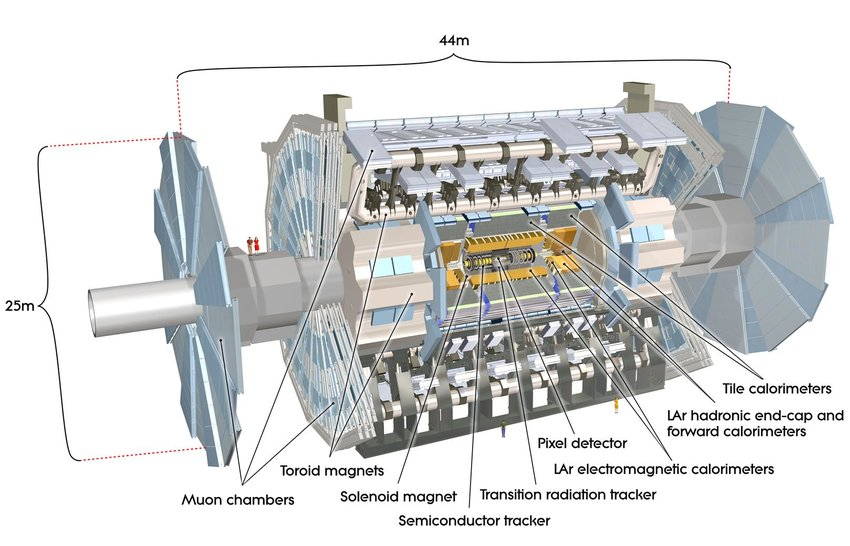
\includegraphics[height=7cm,keepaspectratio]{ATLAS.jpg}
  \caption[ATLAS検出器]{ATLAS検出器の全体図[\cite{ATLAS}]}
  \label{fig:ATLAS}
\end{figure}



ATLAS(A Troidala LHC ApparataS)実験はLHCの衝突点の一つに設置されている汎用型の検出器である。



\subsection{内部秘蹟検出器}

\subsection{カロリメータ}

\subsection{ミューオン検出器}









\section{HL-LHCアップグレード}



\newpage
